\documentclass[12pt]{article}
\usepackage{graphicx}
%\documentclass[journal,12pt,twocolumn]{IEEEtran}
\usepackage[none]{hyphenat}
\usepackage{graphicx}
\usepackage{listings}
\usepackage[english]{babel}
\usepackage{graphicx}
\usepackage{caption} 
\usepackage{hyperref}
\usepackage{booktabs}
\usepackage{amssymb}
\def\inputGnumericTable{}
\usepackage{color}                                            %%
    \usepackage{array}                                            %%
    \usepackage{longtable}                                        %%
    \usepackage{calc}                                             %%
    \usepackage{multirow}                                         %%
    \usepackage{hhline}                                           %%
    \usepackage{ifthen}
\usepackage{array}
\usepackage{amsmath}   % for having text in math mode
\usepackage{listings}
\lstset{
language=tex,
frame=single, 
breaklines=true
}
  %Following 2 lines were added to remove the blank page at the beginning
\usepackage{atbegshi}% http://ctan.org/pkg/atbegshi
\AtBeginDocument{\AtBeginShipoutNext{\AtBeginShipoutDiscard}}
%
%New macro definitions
\newcommand{\mydet}[1]{\ensuremath{\begin{vmatrix}#1\end{vmatrix}}}
\providecommand{\brak}[1]{\ensuremath{\left(#1\right)}}
%\providecommand{\norm}[1]{\left\lVert#1\right\rVert}
\newcommand{\solution}{\noindent \textbf{Solution: }}
\newcommand{\myvec}[1]{\ensuremath{\begin{pmatrix}#1\end{pmatrix}}}
\let\vec\mathbf
\begin{document}

\begin{center}
\title{\textbf{Vector Algebra}}
\date{\vspace{-5ex}} %Not to print date automatically
\maketitle
\end{center}
\setcounter{page}{1}
\section*{11$^{th}$ Maths - Chapter 10}
This is Problem-12 from Exercise 10.4
\begin{enumerate}
    \item Find the equation of the line passing through the point of intersection of the lines $4x + 7y - 3 = 0$ and $2x - 3y + 1 = 0$ that has equal intercepts on the axes.\\
    \solution \\
    Given lines can be written in the form of n$^{T}$x = $c$
   \\Therefore,\\ \begin{align}
       \myvec{4&7}x=3
   \end{align} 
   \begin{align}
       \myvec{2&-3}x=-1
   \end{align}\\
   Now, line equation that has equal intercepts on the axes is
   \begin{align}
       \myvec{1 & 1}x=c
   \end{align}
   Solving equations (1) and (2)\\augumented matrix is
  \begin{align}
\begin{pmatrix}
    4 & 7 & 3 \\ \\
    2 & -3 & -1
  \end{pmatrix}
\end{align}
$R_1 \leftarrow 4 R_1$
\begin{align}
\begin{pmatrix}
    1 & \frac{7}{4} & \frac{3}{4} \\ \\
    2 & -3 & -1
  \end{pmatrix}
\end{align}
$R_2 \leftarrow R_2 - 2R_1$
\begin{align}
\begin{pmatrix}
    1 & \frac{7}{4} & \frac{3}{4} \\ \\
    0 & \frac{-13}{2} & \frac{-5}{2}
  \end{pmatrix}
\end{align}
$R_2 \leftarrow \frac{-2}{13}R_2$
\begin{align}
\begin{pmatrix}
    1 & \frac{7}{4} & \frac{3}{4} \\ \\
    0 & 1 & \frac{5}{13}
  \end{pmatrix}
\end{align}
$R_1 \leftarrow R_1-\frac{7}{4}R_2$
\begin{align}
\begin{pmatrix}
    1 & 0 & \frac{1}{13} \\ \\
    0 & 1 & \frac{5}{13}
  \end{pmatrix}
\end{align}
Therfore, $x = \myvec{\frac{1}{13}\\ \\ \frac{5}{13}}$ Also this point lies on the equation (3)\\
\begin{center}
    $\myvec{1 & 1}\myvec{\frac{1}{13} \\ \\ \frac{5}{13}} = c$
    \vspace{\baselineskip}\\
    $\frac{1}{13}+\frac{5}{13} = c$
     \vspace{\baselineskip}\\
    Therefore, the equation is $\myvec{1&1}x=\frac{6}{13}$
\end{center}
\begin{figure}
    \centering
	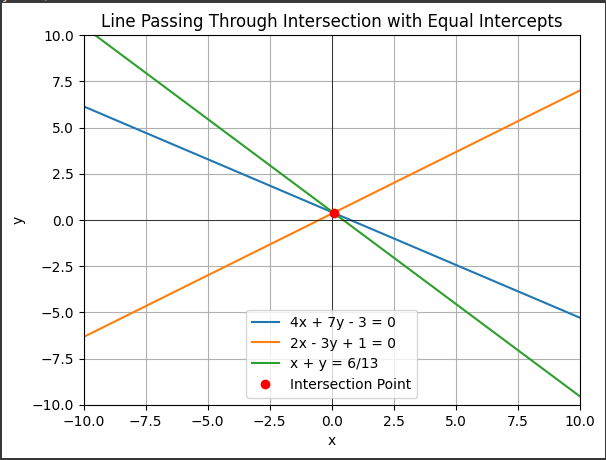
\includegraphics[width=\columnwidth]{stline.png}
    \caption{Straight Lines}
    \label{fig:enter-label}
\end{figure}
\end{enumerate}
\end{document}
